% This LaTeX was auto-generated from MATLAB code.
% To make changes, update the MATLAB code and export to LaTeX again.

\documentclass{article}


\usepackage{lmodern}
\usepackage{graphicx}
\usepackage{color}
\usepackage{hyperref}
\usepackage{amsmath}
\usepackage{amsfonts}
\usepackage{epstopdf}
\usepackage[table]{xcolor}
\usepackage{matlab}

\sloppy
\epstopdfsetup{outdir=./}
\graphicspath{ {./HW4_images/} }

\begin{document}

\matlabtitle{Homework a\# 4: Computational Physics}


\vspace{1em}
\matlabheadingtwo{Name: Pablo Lopez}

\matlabheadingtwo{October 7th, 2020}


\vspace{1em}

\vspace{1em}
\matlabheading{Problem 1}

\begin{par}
\begin{flushleft}
b) Using the adaptive Runge-Kutta technique, we can easily solve the resulting equation:
\end{flushleft}
\end{par}

\begin{par}
$$\left\lbrace \begin{array}{ll}
\frac{\mathrm{dr}}{\mathrm{dt}}=r\left(a-r^2 \right) & \\
\frac{d\theta \;\;}{\mathrm{dt}}=-1 & 
\end{array}\right.$$
\end{par}


\begin{par}
\begin{flushleft}
in which we include the system of uncoupled differential equations.
\end{flushleft}
\end{par}

\begin{par}
\begin{flushleft}
In order to solve it, we must then define the parameters and initial conditions for our system:
\end{flushleft}
\end{par}

\begin{matlabcode}
A = 4;
ms=3;
tspan = [0 3.5];
yinit=[0.0001,0.5*pi;0.1,0.5*pi;0.5,0.5*pi;1.5,0.5*pi;4.0,0.5*pi];
\end{matlabcode}

\begin{par}
\begin{flushleft}
where we define a 5x2 matrix to automatize the solutions for several initial conditions. In the same manner we automatize the marker selection:
\end{flushleft}
\end{par}

\begin{matlabcode}
chars=["-o","-x","-s","-.","-"];
\end{matlabcode}


\matlabheadingthree{Case a\textgreater{}0:}

\begin{par}
\begin{flushleft}
Then, we can use ode45 to solve the system, plot the solutions in the same figure and save it :
\end{flushleft}
\end{par}

\begin{matlabcode}
for ii=1:size(yinit,1)
    [t,y] = ode45(@(t,y) odefcn(t,y,A), tspan, yinit(ii,:));
    plot(t,y(:,1),chars(ii),'MarkerSize',ms)
    hold all
end
title('Hopf model theta solution for a=4');

legend('r0=0.0001','r0=0.1','r0=0.5','r0=1.5','r0=4');
box on

ax=gca;
ax.FontSize=12;

xlabel('t');
ylabel('r(t)');

%saveas(gcf,'HW4_1b_loop_a4','epsc');

hold off
\end{matlabcode}
\begin{center}
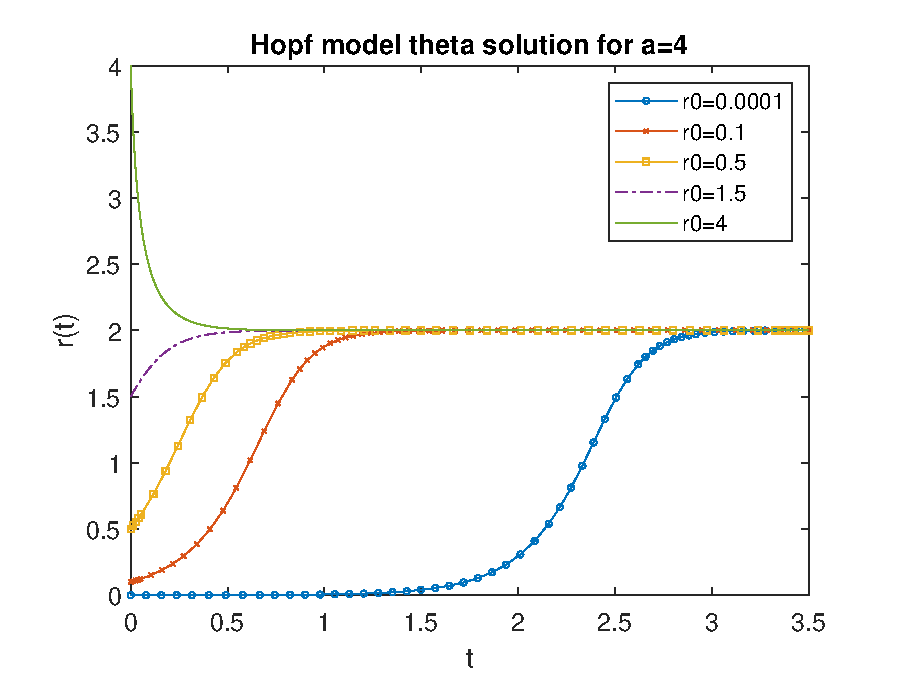
\includegraphics[width=\maxwidth{56.196688409433015em}]{figure_0.eps}
\end{center}

\begin{par}
\begin{flushleft}
As we can see in this figure below, the solutions approach $\sqrt{4}$ for any initial set of values.
\end{flushleft}
\end{par}


\begin{par}
\begin{flushleft}
Now, lets try with a couple different values for $a$:
\end{flushleft}
\end{par}

\begin{matlabcode}
%For a=2
A = 2;
ms=3;
tspan = [0 6];
yinit=[0.0001,0.5*pi;0.1,0.5*pi;0.5,0.5*pi;1.5,0.5*pi;4.0,0.5*pi];
for ii=1:size(yinit,1)
    [t,y] = ode45(@(t,y) odefcn(t,y,A), tspan, yinit(ii,:));
    plot(t,y(:,1),chars(ii),'MarkerSize',ms)
    hold all
end
title('Hopf model theta solution for a=2');

legend('r0=0.0001','r0=0.1','r0=0.5','r0=1.5','r0=4');
box on

ax=gca;
ax.FontSize=12;

xlabel('t');
ylabel('r(t)');

%saveas(gcf,'HW4_1b_loop_a2','epsc');

hold off
\end{matlabcode}
\begin{center}
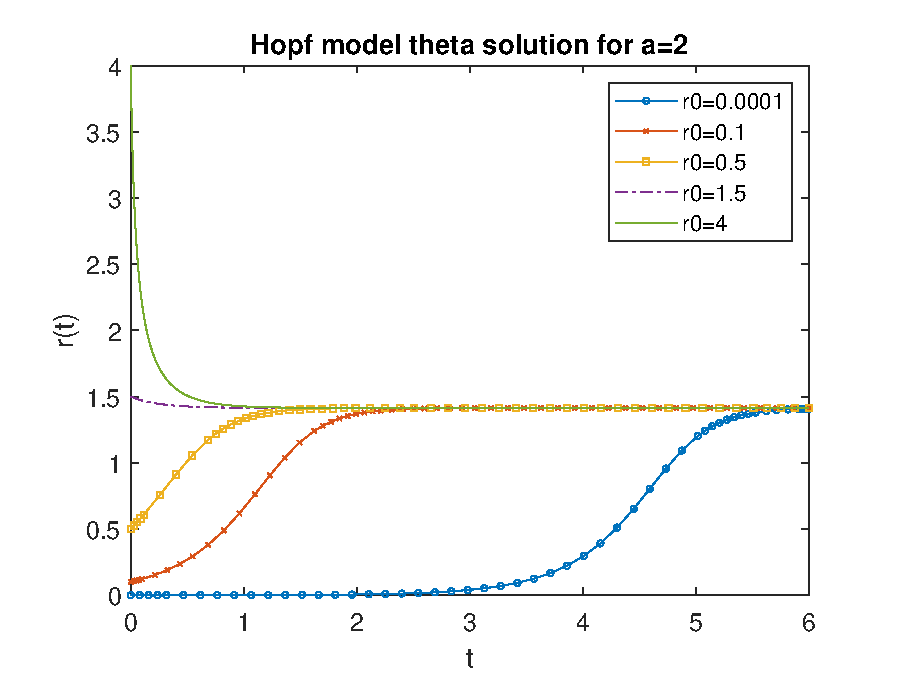
\includegraphics[width=\maxwidth{56.196688409433015em}]{figure_1.eps}
\end{center}

\begin{par}
\begin{flushleft}
Again, the function approaches $r=\sqrt{\;2}$.
\end{flushleft}
\end{par}


\begin{par}
\begin{flushleft}
Finally, lets try $a=0\ldotp 25$:
\end{flushleft}
\end{par}

\begin{matlabcode}
%For a=0.25
A = 0.25;
ms=3;
tspan = [0 40];
yinit=[0.0001,0.5*pi;0.1,0.5*pi;0.5,0.5*pi;1.5,0.5*pi;4.0,0.5*pi];
for ii=1:size(yinit,1)
    [t,y] = ode45(@(t,y) odefcn(t,y,A), tspan, yinit(ii,:));
    plot(t,y(:,1),chars(ii),'MarkerSize',ms)
    hold all
end
title('Hopf model theta solution for a=1/4');

legend('r0=0.0001','r0=0.1','r0=0.5','r0=1.5','r0=4');
box on

ax=gca;
ax.FontSize=12;

xlabel('t');
ylabel('r(t)');

%saveas(gcf,'HW4_1b_loop_a025','epsc');

hold off
\end{matlabcode}
\begin{center}
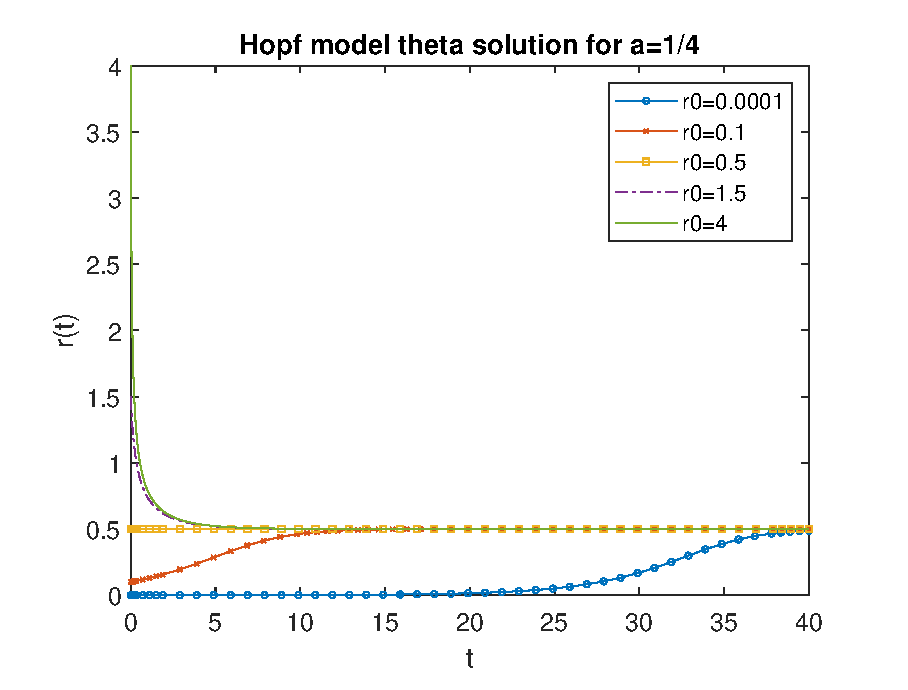
\includegraphics[width=\maxwidth{56.196688409433015em}]{figure_2.eps}
\end{center}

\begin{par}
\begin{flushleft}
Once again, the function approaches $r=\sqrt{\;0\ldotp 25}$.
\end{flushleft}
\end{par}

\begin{par}
\begin{flushleft}
We can clearly see that for values closer to zero, the time that it takes to converge to $\sqrt{a}$ is longer.
\end{flushleft}
\end{par}


\begin{par}
\begin{flushleft}
Case a\textless{}0:
\end{flushleft}
\end{par}

\begin{matlabcode}
%For a=-4
A = -4.0;
ms=3;
tspan = [0 1.5];
yinit=[0.0001,0.5*pi;0.1,0.5*pi;0.5,0.5*pi;1.5,0.5*pi;4.0,0.5*pi];
for ii=1:size(yinit,1)
    [t,y] = ode45(@(t,y) odefcn(t,y,A), tspan, yinit(ii,:));
    plot(t,y(:,1),chars(ii),'MarkerSize',ms)
    hold all
end
title('Hopf model theta solution for a=-4');

legend('r0=0.0001','r0=0.1','r0=0.5','r0=1.5','r0=4');
box on

ax=gca;
ax.FontSize=12;

xlabel('t');
ylabel('r(t)');

%saveas(gcf,'HW4_1b_loop_an4','epsc');

hold off
\end{matlabcode}
\begin{center}
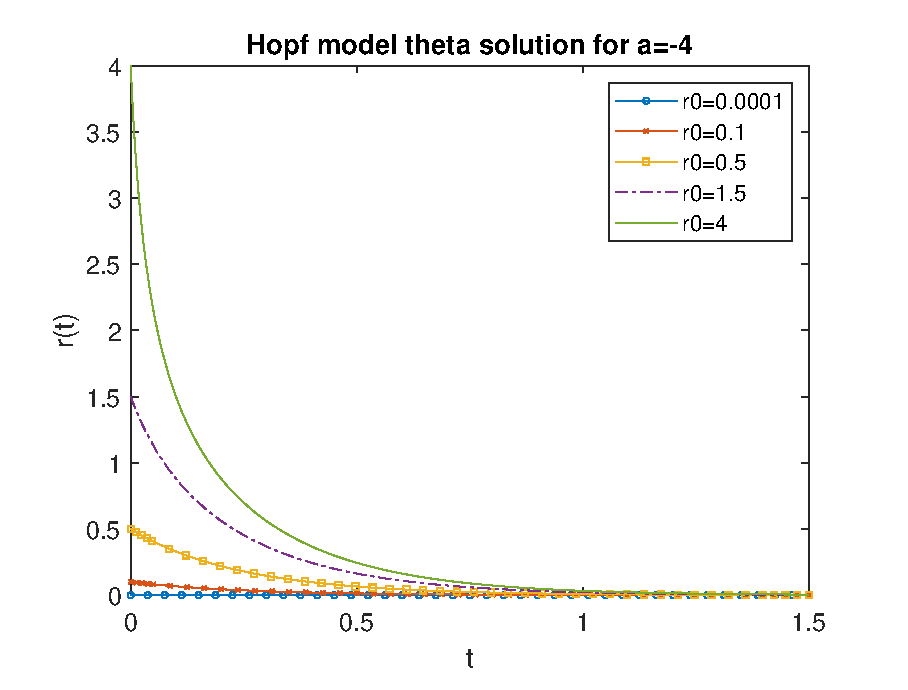
\includegraphics[width=\maxwidth{56.196688409433015em}]{figure_3.eps}
\end{center}

\begin{par}
\begin{flushleft}
In the case $a<0$, we see a completely different behavior, as we showed in part a. In this case, the system always converges to $r=0\ldotp$ The only difference the starting parameters have is on how fast the approach to zero is. 
\end{flushleft}
\end{par}


\matlabheadingtwo{Theta equation}

\begin{par}
\begin{flushleft}
The simpler to analyze is the $\theta \;$equation as it clearly represents a constant decrease over time. 
\end{flushleft}
\end{par}

\begin{matlabcode}
A = 0.25;
ms=3;
tspan = [0 40];
yinit=[0.0001,0.5*pi;0.1,0.5*pi;0.5,0.5*pi;1.5,0.5*pi;4.0,0.5*pi];
for ii=1:size(yinit,1)
    plot(t,y(:,2),chars(ii),'MarkerSize',ms)
    hold all
end
title('Hopf model theta solution for a=1/4');

legend('r0=0.0001','r0=0.1','r0=0.5','r0=1.5','r0=4');
box on

ax=gca;
ax.FontSize=12;

xlabel('t');
ylabel('r(t)');

%saveas(gcf,'HW4_1b_loop_theta_a025','epsc');
hold off
\end{matlabcode}
\begin{center}
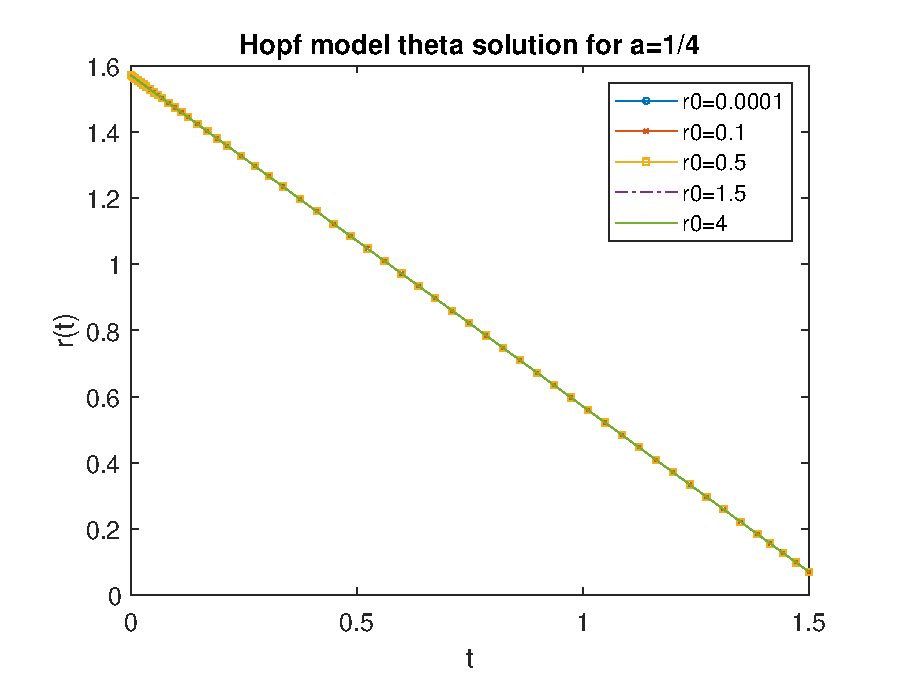
\includegraphics[width=\maxwidth{56.196688409433015em}]{figure_4.eps}
\end{center}

\begin{par}
\begin{flushleft}
Clearly, no matter what parameters we choose, we will always end up with the same behavior.
\end{flushleft}
\end{par}


\begin{par}
\begin{flushleft}
In order to implement any of the code parts above, we will define the following function:
\end{flushleft}
\end{par}

\begin{matlabcode}
function dydt = odefcn(t,y,A)
    dydt = zeros(2,1);
    dydt(1) = y(1)*(A-y(1)^2);
    dydt(2) = -1;
end
\end{matlabcode}

\end{document}
